%%%%%%%%%%%%%%%%%%%%%%%%%%%%%%%%%%%%%%%%%%%%%%%%%%%%%%%%%%%%%%%%%
%%% %
%%% % weiiszablon.tex
%%% % The Faculty of Electrical and Computer Engineering
%%% % Rzeszow University Of Technology diploma thesis Template
%%% % Szablon pracy dyplomowej Wydziału Elektrotechniki 
%%% % i Informatyki PRz
%%% % June, 2015
%%%%%%%%%%%%%%%%%%%%%%%%%%%%%%%%%%%%%%%%%%%%%%%%%%%%%%%%%%%%%%%%%

\documentclass[12pt,twoside]{article}

\usepackage[section]{placeins}
\usepackage{weiiszablon}

\author{Krzysztof Lang}

% np. EF-123456, EN-654321, ...
\studentID{EF-148853}

\title{Implementacja wybranych algorytmów wypełniania brakujących wartości, dla strumieni dużych zbiorów danych}
\titleEN{Implemetation of selected missing value filling algorithms for large data sets}


%%% wybierz rodzaj pracy wpisując jeden z poniższych numerów: ...
% 1 = inżynierska	% BSc
% 2 = magisterska	% MSc
% 3 = doktorska		% PhD
%%% na miejsce zera w linijce poniżej
\newcommand{\rodzajPracyNo}{2}


%%% promotor
\supervisor{dr Michał Piętal}
%% przykład: dr hab. inż. Józef Nowak, prof. PRz

%%% promotor ze stopniami naukowymi po angielsku
\supervisorEN{Michał Piętal, PhD}

\abstract{Dla poprawnej analizy danych ważna jest ich kompletność.
Istnieje wiele sposobów radzenia sobie z brakującymi danymi.
Najprostsze metody opierające się między innymi na średniej bądź najczęściej występującej wartości w wielu przypadkach
mogą negatywnie wpłynąć na skuteczność analizy. Niniejsza praca ma na celu przeanalizować skuteczność uzupełniania
brakujących danych z użyciem bardziej zaawansowanych metod opierających się na wykorzystaniu uczenia maszynowego.
Te metody mają na celu wypełnić brakujące dane wartościami dużo bardziej zbliżonymi do rzeczywistych,
minimalizując negatywny wpływ na skuteczność późniejszej analizy danych.}
\abstractEN{For correct data analysis, completeness is important. There are many ways to deal with missing data.
The simplest methods based on, among other things, nthe average or the most frequently occurring value
in many cases can negatively affect the effectiveness of the analysis. This paper aims to analyze the effectiveness
of filling in missing data using more advanced methods based on the use of machine learning.
These methods are designed to fill in missing data with values much closer to the actual data,
minimizing the negative impact on the effectiveness of subsequent data analysis.}

\begin{document}

% strona tytułowa
\maketitle

\blankpage

% spis treści
\tableofcontents
\clearpage
\blankpage


\section{Wstęp}
\clearpage


\section{Wprowadzenie do wypełniania brakujących wartości}

\subsection{Rys historyczny}
\subsection{Na czym polega wypełnianie brakujących wartości}
\subsection{Korzyści i zagrożenia}
\subsection{Perspektywy na przyszłość}
\clearpage


\section{Omówienie narzędzi i danych}

\subsection{Python}

Do przygotowania programu wykorzystanego do przeprowadzenia badań wybrano język Python.
Jest to język wysokiego poziomu, charakteryzujący się prostą składną i wysoką przejrzystoścą kodu.
Programy nie muszą być kompilowane przed uruchomieniem, co znacznie przyśpiesza proces prototypowania i debugowania.
Oznacza to też że Python jest wolniejszy od wielu innych języków, jednak w przypadku niniejszej pracy nie ma to znaczenia.
Dostępna ogromna ilość gotowych bibliotek służących do obróbki i analizy danych znacząco uprościła przygotowanie programu.
Podczas pisania kodu trzymano się dobrych praktyk, stosowano wytyczne zawarte w PEP8.
\subsection{Visual Studio Code}

Jako środowisko programowania wybrano "Microsoft Visual Studio Code".
Jest to darmowy edytor kodu obsługujący wiele języków.
Ze wzglądu na otwartość kodu, dostępne jest wiele rozszerzeń do programu,
które znacznie ułatwiają tworzenie nawet skomplikowanych projektów.
W celu umożliwienia pracy nad programem z wielu urządzeń
oraz dla zachowania pełnej historii tworzenia programu wykorzystano integrację "Visual Studio Code" z repozytorium GitHub.
\subsection{Biblioteki}
\subsubsection{Pandas}
\subsubsection{NumPy}
\subsubsection{Scikit}
\subsubsection{EasyGUI}
\subsection{Źródła danych}

\subsubsection{Użyte repozytoria danych}

Aby wyniki badań niosły ze sobą odpowiednią wartość merytoryczną,
potrzebne są odpowiednie zbiory danych na których zostaną przeprowadzone testy
W celu znalezienia odpowiednich zbiorów danych, przyjęto następujące założenia:
\begin{itemize}[label=-,labelsep=0.4cm, leftmargin=1.25cm]
    \item zbiór danych musi być wystarczająco duży,
    \item zbiór danych musi zawierać odpowiedniż ilość atrybutów aby modele decyzyjne miały
    do dyspozycji wystarczającą ilość danych uczących,
    \item atrybuty powinny zawierać różnorodne typy danych w celu przetestowania wypełniania zarówno danych
    liczbowych (całkowitych i zmiennoprzecinkowych) jak i kategorycznych,
    \item zbiór danych nie może mieć pustych wartości.
\end{itemize}
Do wyszukania odpowiednich zbiorów danych wykorzystano narzędzie "Google Dataset Search".
Z jego pomocą wybrano 2 zbiory danych z róźnych dziedzin.
Po uprzedniej ich obróbce zostały wykorzystane do przeprowadzenia testów algorytów wypełniania.
\subsubsection{Adult Data Set}

Zbiór danych "Adult Data Set" zawiera dane ze spisu ludności przeprowadzonego w roku 1994 w Stanach Zjednoczonych.
Jest szeroko wykorzystywany do testowania uczenia maszynowego.
Zawiera ponad 30000 rekordów i 15 atrybutów. \cite{adult} Opis atrybutów:
\begin{itemize}[label=-,labelsep=0.4cm, leftmargin=1.25cm]
    \item age: wiek spisanej osoby, liczba całkowita,
    \item workclass: rodzaj zatrudnienia, dane kategoryczne, 8 możliwych wartości,
    \item fnlwgt: jaka proporcja populacji ma identyczny zestaw pozostałych wartości, liczba całkowita,
    \item education: osiągnięty poziom edukacji, dane kategoryczne, 16 możliwych wartości,
    \item education-num: osiągnięty poziom edukacji zakodowany jako liczba całkowita,
    \item martial-status: status matrymonialny, dane kategoryczne, 7 możliwych wartości,
    \item occupation: zawód, dane kategoryczne, 14 możliwych wartości,
    \item relationship: rola w związku, dane kategoryczne, 6 możliwych wartości,
    \item race: klasyfikacja rasowa, dane kategoryczne, 5 możliwych wartości,
    \item sex: płeć, dane kategoryczne, 2 możliwe wartości,
    \item capital-gain: zysk kapitału w zwiazku z inwestycjami, liczba całkowita,
    \item capital-gain: strata kapitału w zwiazku z inwestycjami, liczba całkowita,
    \item hours-per-week: ilość godzin pracujących w tygodniu, liczba całkowita,
    \item native-country: kraj pochodzenia, dane kategoryczne, 41 możliwych wartości,
    \item attribute: czy osoba zarabia powyżej czy poniżej 50000\$ rocznie.
\end{itemize}
Ten zbiór danych został wybrany ze względu na występowanie zarówno atrybutów liczbowych jak i kategorycznych,
zadowalajacą ilość rekordów oraz atrybutów.
Ma na celu przetestowanie skuteczności działania algorytmów do wypełniania brakujących miejsc
w zbiorach danych z brakami w danych o różnych typach.
Nie wymaga dodatkowej obróbki przed rozpoczęciem testów. 
\subsubsection{Stock Exchange Data}

Zbiór danych "Stock Exchange Data" zawiera informacje o cenach akcji na giełdach w różnych krajach w latach 1965-2021.
Dane zostały zebrane z "Yahoo Finance", posiadającego dane o giełdzie z wielu lat w wielu krajach.
Posiada ponad 100000 rekordów i 9 atrybutów. \cite{stock} Opis atrybutów:
\begin{itemize}[label=-,labelsep=0.4cm, leftmargin=1.25cm]
    \item Index: symbol wskazujacy z jakiej giełdy pochodzą dane, dane kategoryczne, 5 możliwych wartości,
    \item Date: data obserwacji, dane kategoryczne,
    \item Open: cena akcji podczas otwarcia, liczba wymierna,
    \item High: najwyższa cena w ciągu dnia, liczba wymierna,
    \item Low: najniższa cena w ciągu dnia, liczba wymierna,
    \item Close: cena akcji w momencie zamknięcia, liczba wymierna,
    \item Adj Close: cena akcji w momencie zamknięcia skorygowana o podziały jak i dywidendy, liczba wymierna,
    \item Volume: liczba akcji będących przedmiotem obrotu w ciągu dnia sesyjnego, liczba całkowita,
    \item CloseUSD: cana akcji w momencie zamknięcia wyrażona w dolarach amerykańskich
\end{itemize}
Ten zbiór danych został wybrany ze względu na bardzo popularną kategorię danych, to jest dane finansowe.
Ma na celu przetestowanie skuteczności działania algorytmów w przypadku danych numerycznych,
w szególności liczb wymiernych.
W celu lepszego przygotowania do testów zakodowano kolumnę "Data" z wykorzystaniem "label encoding",
to jest zamiany danych na postać numeryczną.
Usunięto też rekordy posiadające wartość "0" w kolumnie "Volume".
Ich duża ilość (ponad 30\%) mogła by negatywnie wpłynąć na uczenie modeli decyzyjnych.
W wyniku tego zmniejszono liczbę rekordów do ponad 62000,
co wciąż jest ilością spełniajacą założenia dla zbiorów danych.


\clearpage
\section{Opis przygotowanego programu}
\subsection{Założenia i realizacja}
Założono, że program ma rtealizować 3 zadania:

\begin{enumerate}[label=\arabic*), leftmargin=1.25cm]
    \item Przygotować dane do wypełniania poprzez sztuczne utworzenie brakujacych wartości.
    \item Wypełnić brakujące wartości z wykorzystaniem wybranych algorytmów.
    \item Ocenić skuteczność wypełniania w celu porównania algorytmów.
\end{enumerate}

Poszczególne zadania zrealizowano jako osobne moduły.

Przyjęto też następujące założenia:

\begin{enumerate}[label=\arabic*), leftmargin=1.25cm]
    \item Wykorzystanym językiem ma być Python.
    \item Program ma być napisany zgodnie z paradygmatem programowania obiektowego.
    \item Poszczególne klasy mają być zawarte w osobnych plikach.
    \item Interakcja z programem ma opierać się o prosty interfejs graficzny.
    \item Dostęp do wszystkich modułów programu ma być zapewniony z jednego miejsca.
    \item Pliki wygenerowane przez jeden moduł mają być przygotowane w sposób umożliwiający
    wykorzystanie ich przez kolejny. Oprócz odpowiedniego formatowania wewnątrz pliku,
    oznacza to przyjęcie konwencji nazewnictwa plików opartej o prefiksy i sufiksy.
\end{enumerate}

Program składa się z następujacych plików:

\begin{itemize}[label=-,labelsep=0.4cm, leftmargin=1.25cm]
    \item mgr\_main.py: główny plik nie zawierający żadnej klasy, odpowiadający za wybór modułu do uruchomienia,
    i uruchomienie odpowiedniego modułu po wybraniu,
    \item mgr\_nan\_gen" plik zawierajacy klasę "NanGen", odpowiadającą za realizację modułu przygotowujacego plik,
    \item mgr\_fill.py: plik zawierający klasę "Fill", odpowiadającą za realizację modułu wypełniajacego brakuące dane,
    \item mgr\_data.py: plik zawierający klasę "Data",
    odpowiadającą za wybranie pliku do wypełnienia i przygotowanie do do dalszej obróbki, oraz klasę "PrepareData",
    odpowiadającą za przygotowanie danych do przekazania silnikowi uczenia maszynowego celem wypełnienia
    oraz późniejszemu przywróceniu danym ich pierwotnego wyglądu
    \item mgr\_di.py: plik zawierjący klasę DownImpu,
    odpowiadającą za przygotowanie danych dla algorytmu "Downward Imputation"
    \item mgr\_temp\_fill: plik zawierający klasę "TempFill", odpowiadającą za tymczasowe wypełnianie brakujących miejsc,
    potrzebne podczas przygotowywania danych dla algorytmu "Prostego"
    \item mgr\_acc: plik zawierający klasę "AccuracyTester", odpowiadającą za obliczanie skuteczności wypełniania danych
\end{itemize}

Wykorzystując narzędzie "auto-py-to-exe", utworzono plik "mgr\_suite.exe",
pozwalajacy uruchomić program bez konieczności instalowania interpretera Python i potrzebnych bibliotek.

\subsection{Działanie programu}
Poniżej zaprezentowano działanie programu na przykładzie pliku data\_stock.csv.
Zostanie on najpierw przygotowany do testów,
następnie brakujace dane zostaną wypełnione z wykorzystaniem jednego z algorytmów,
po czym zostanie obliczona dokładność tego wypełnienia.
\subsubsection{Uruchomienie}
Po uruchomieniu "mgr\_suite.exe" wyświetlone zostaje okno służące do wyboru modułu, pokazane na rysunku \ref{Fig:main}.

\begin{figure}[ht]
	\centering
	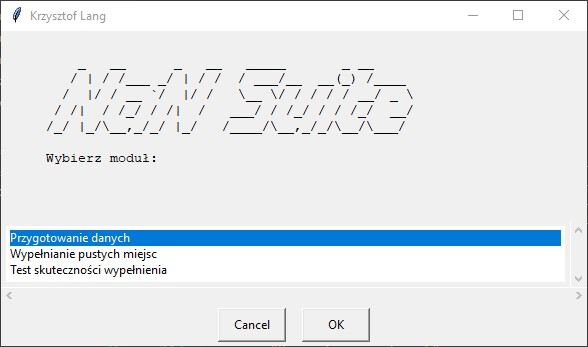
\includegraphics[width=12cm]{img/01.jpg}
	\caption{Główne okno programu, pozwalajace na wybór modułu do uruchomienia}
\label{Fig:main}
\end{figure}

\subsubsection{Przygotowanie danych}

Pierwszy moduł odpowiada za przygotowanie danych do wypełniania poprzez usunięcie losowych wartości ze zbioru danych.
Pierwszym krokiem jest wybranie pliku który ma zostać przygotowany
z użyciem okna pokazanego na rysunku \ref{Fig:gen_file}.
Lista plików generowana jest na podstawie plików znajdujących się
w tym samym folderze co uruchamiany program spełniających założony format nazwy.
Założono, że pliki które nadają się do wypełnienia mają być zapisane w formacie CSV,
natomiast nazwa zaczynać się ma od prefiksu "data\_" i nie posiadać żadnych sufiksów.

\begin{figure}[ht]
	\centering
	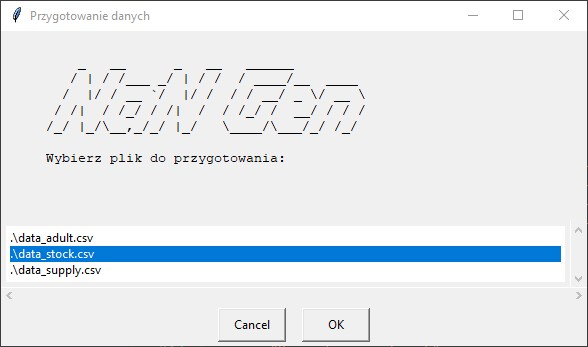
\includegraphics[width=12cm]{img/02.jpg}
	\caption{Okno wyboru pliku do przygotowania}
\label{Fig:gen_file}
\end{figure}

Następnie wybrane z listy zostają kolumny w których maja zostać usunięte dane.
Wyboru dokonuje się z użyciem okna pokazanego na rysunku \ref{Fig:gen_col}.
Kolumny do wyboru zaczerpnięte są bezpośrednio z załadowanego wcześniej pliku.
Wybrać można dowolną ilość, lecz zalecane jest poniżej 50\%.

\begin{figure}[ht]
	\centering
	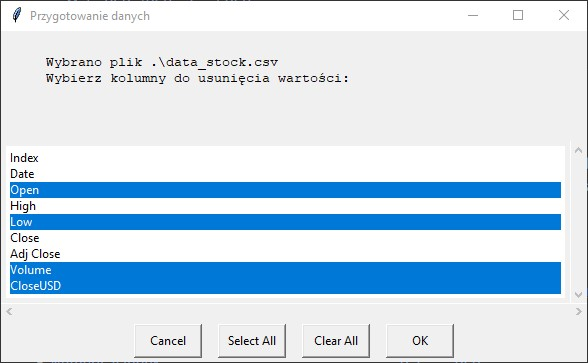
\includegraphics[width=12cm]{img/03.jpg}
	\caption{Okno wyboru kolumn}
\label{Fig:gen_col}
\end{figure}

W wybranych kolumnach zostaje usunięte od 5\%
do 15\% wartości - dla każdej kolumny ilość jest losowana.
Dodatkowo stworzony zostaje plik przechowujęcy informacje które wartości zostały usunięte.
Ta informacja zostaje później wykorzystana do oceny skuteczności wypełnienia zbioru danych.
Po zakończeniu usuwania wartości wyświetlone zostaje okno z podsumowaniem jak na rysunku \ref{Fig:gen_end}.
Nazwa utworzonego pliku z gotowymi danymi tworzona jest
poprzez dodanie sufiksu "\_holes\_X" do nazwy oryginalnego pliku, gdzie X to kolejna liczba naturalna.
Umożliwia to tworzenie plików z danymi usuniętymi z różnych zestawów kolumn bez konieczności ręcznej zmiany ich nazw.
Nazwa pliku z informacją które dane zostały usunięte tworzona jest
przez dodanie sufiksu "\_journal" do nazwy oryginalnego pliku.

\begin{figure}[ht]
	\centering
	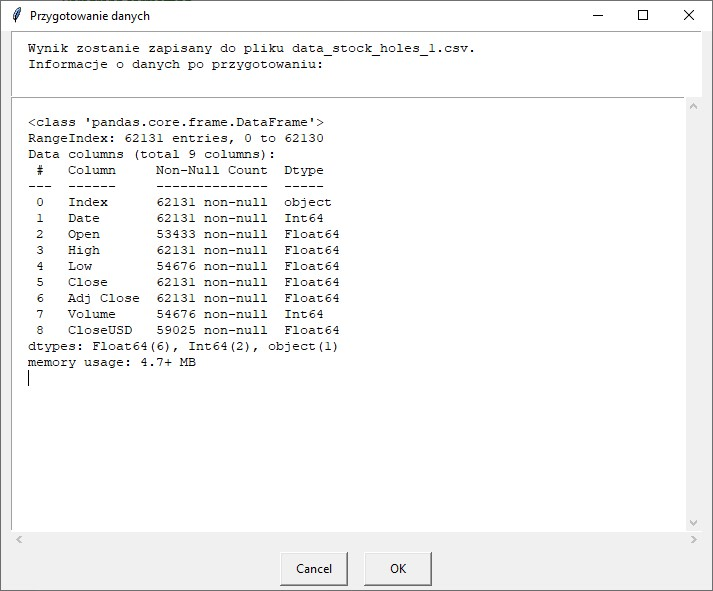
\includegraphics[width=12cm]{img/04.jpg}
	\caption{Okno z podsumowaniem}
\label{Fig:gen_end}
\end{figure}

\subsubsection{Wypełnianie brakujących wartości}

Drugi moduł służy do wypełniania brakujacych wartości w zbiorze danych z użyciem wybranego algorytmu. 

Najpierw należy wskazać plik który ma zostać wypełniony z użyciem okna wyboru pokazanego na rysunku \ref{Fig:fill_file}.
Tak jak wcześniej, lista tworzona jest na podstawie plików w folderze i przyjętej konwencji nazewnictwa plików.
Wyświetlane są wyłącznie pliki posiadające sufiks "\_holes\_X" w nazwie, bez kolejnych sufiksów.

\begin{figure}[ht]
	\centering
	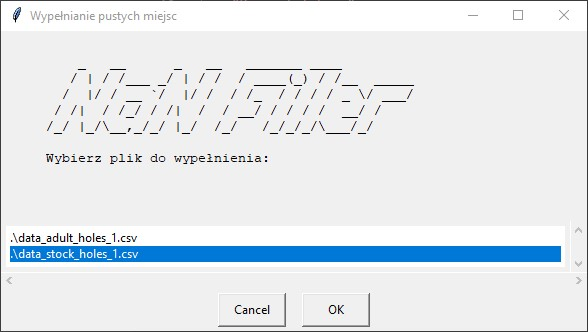
\includegraphics[width=12cm]{img/05.jpg}
	\caption{Okno wyboru pliku do wypełnienia}
\label{Fig:fill_file}
\end{figure}

Następnie z użyciem okna jak na rysunku \ref{Fig:fill_alg}
wybrany zostaje algorytm który ma zostać wykorzystany do wypełniania brakujących wartości.
Wyświetlona zostaje też nazwa wybranego wcześniej pliku w celu uniknięcia błędu wybrania niewłaściwego pliku.

\begin{figure}[ht]
	\centering
	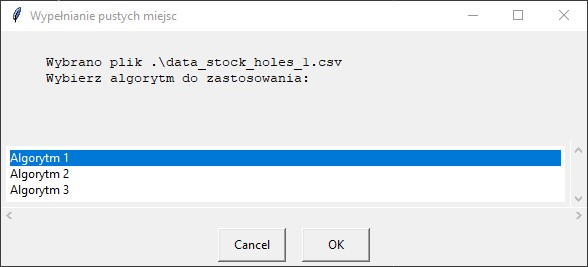
\includegraphics[width=12cm]{img/06.jpg}
	\caption{Okno wyboru algorytmu}
\label{Fig:fill_alg}
\end{figure}

Puste miejsca zostają wypełnione z wykorzystaniem wybranego algorytmu.
Dokładny sposób działania algorytmów zostanie opisany w kolejnych rozdziałach.
Po zakończeniu wypełniania wyświetlone zostaje podsumowanie jak na rysunku \ref{Fig:fill_end}.
Nazwa pliku wynikowego tworzona jest poprzez dodanie sufixu "\_filled\_Y", gdzie Y to nazwa wybranego algorytmu.

\begin{figure}[ht]
	\centering
	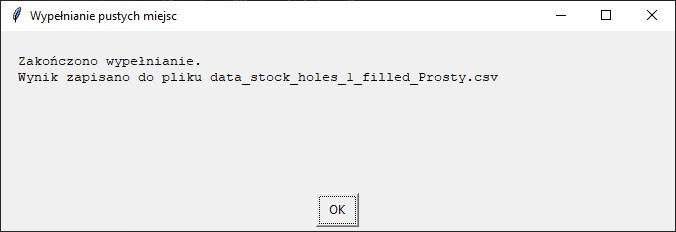
\includegraphics[width=12cm]{img/07.jpg}
	\caption{Okno z podsumowaniem wypełniania}
\label{Fig:fill_end}
\end{figure}

\subsubsection{Sprawdzenie skuteczności wypełniania}

Ostatni moduł odpowiada za wygenerowanie danych,
które można wykorzystać do oceny skuteczności wypełniania brakujących wartości.
Jako wystarczające uznano procent skuteczności wypełniania dla danych kategorycznych i liczb całkowitych
oraz średnie odchylenie bezwzględne dla wszystkich danych liczbowych.
Obie wartości są obliczane dla poszczególnych wypełnionych kolumn.

Jak w przypadku poprzednich modułów, zacząć należy od wyboru pliku który ma zostać poddany analizie.
Wyboru dokonuje się z użyciem okna pokazanego na rysunku \ref{Fig:acc_file}.
Wyświetlane są tylko pliki zawierające słowo "filled" w nazwie, ponieważ takie pliki
posiadają wartości wypełnione za pomocą któregoś algorytmu z użyciem odpowiedniego modułu.

\begin{figure}[ht]
	\centering
	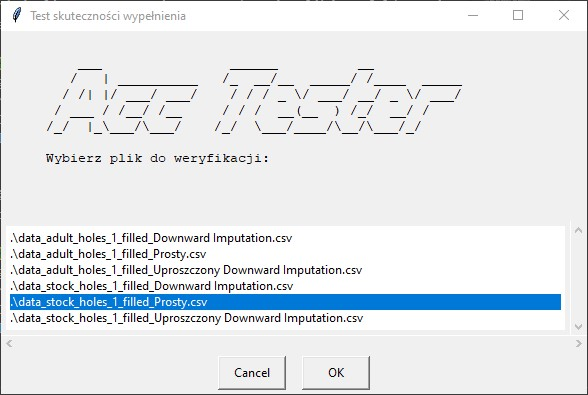
\includegraphics[width=12cm]{img/08.jpg}
	\caption{Okno wyboru pliku do analizy}
\label{Fig:acc_file}
\end{figure}

Z użyciem wybranego pliku, oryginalnego pliku z danymi przed usunięciem losowych danych
oraz pliku z informacją które dane zostały usunięte a następnie wypełnione,
przeprowadzane jest obliczanie skuteczności wypełniania danych.

Obliczenie procentowej skuteczności wypełnienia przebiega następująco:

\begin{enumerate}[label=\arabic*), leftmargin=1.25cm]
    \item Sprawdzenie ilości wypełnianych wartości w danej kolumnie.
    \item Zsumowanie ilości poprawnie wypełnionych danych w kolumnie poprzez porównanie wartości o współrzędnych
    zapisanych w pliku tworzonym podczas przygotowywania danych.
    \item Zastosować wzór \ref{Eq:acc}:
        \begin{equation}
        ACC=\frac{m}{n}\times100\%
        \label{Eq:acc}
        \end{equation}
    gdzie: $ACC$ -- procentowa skuteczność wypełnienia kolumny,
    $m$ -- ilość poprawnie wypełnionych wartości,
    $n$ -- ilość wypełnionych wartości.
\end{enumerate}

Aby obliczyć średnie odchylenie bezwzględne należy zastosować wzór \ref{Eq:aad}:

    \begin{equation}
    AAD=\frac{\sum_{i=1}^{n}|x_i - \hat{x_i}|}{n}
    \label{Eq:aad}
    \end{equation}

gdzie: $AAD$ -- średnie odchylenie bezwzględne dla danej kolumny,
$n$ -- ilość wypełnionych wartości w kolumnie,
$x_i$ -- wartość wypełnionego $i$-tego elementu kolumny,
$\hat{x_i}$ -- oryginalna wartość $i$-tego elementu kolumny.

Po zakończeniu obliczeń, wyświetlane jest podsumowanie jak na rysunku \ref{Fig:acc_end},
a wynik obliczeń zapisywany jest w dwóch plikach

\begin{itemize}[label=-,labelsep=0.4cm, leftmargin=1.25cm]
    \item wyniki obliczania procentowej skuteczności jest zapisywany w pliku o nazwie
    tworzonej przez dodanie do nazwy analizowanego pliku sufiksu "\_aad",
    \item wyniki obliczania średniego odchylenia bezwzględnego jest zapisywany w pliku o nazwie
    tworzonej przez dodanie do nazwy analizowanego pliku sufiksu "\_acc".
\end{itemize}

\begin{figure}[ht]
	\centering
	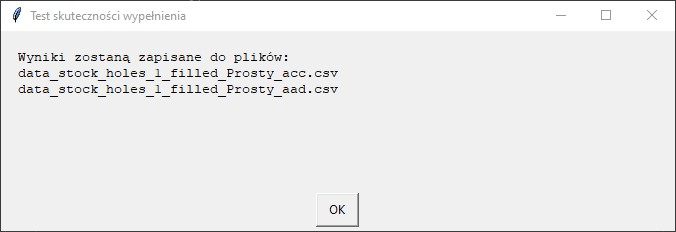
\includegraphics[width=12cm]{img/09.jpg}
	\caption{Okno z podsumowaniem}
\label{Fig:acc_end}
\end{figure}

\clearpage
\section{Implementacja i testy algorytmu}
\subsection{Opis implementacji}
\subsubsection{Alg 1}
\subsubsection{Alg 2}
\subsubsection{Alg 3}
\subsection{Napotkane problemy}
\subsection{Testy algorytmów na wybranych źródłach danych}
\clearpage


\section{Podsumowanie i wnioski końcowe}

\clearpage


\section*{Załączniki}

\addcontentsline{toc}{section}{Załączniki}

\clearpage


\addcontentsline{toc}{section}{Literatura}

\begin{thebibliography}{4}
    \bibitem{adult} archive.ics.uci.edu/ml/datasets/adult. Dostęp 26.02.2023.
    \bibitem{stock} www.kaggle.com/datasets/mattiuzc/stock-exchange-data. Dostęp 26.02.2023.
\end{thebibliography}

\clearpage


\makesummary

\end{document} 
